\documentclass[border=10mm]{standalone}
\usepackage{tikz}
\usetikzlibrary{arrows, shapes.gates.logic.US, shapes.gates.logic.IEC, calc}

\tikzset{
    my-and-gate/.style={
        and gate US, draw, rotate=0, logic gate inputs=nn
    },
    my-xor-gate/.style={
      xor gate US, draw, rotate=0, logic gate inputs=nn
    },
    my-or-gate/.style={
      or gate US, draw, rotate=0, logic gate inputs=nn
    },
    my-branch/.style={
      fill, shape=circle, minimum size=3pt, inner sep=0pt
    },
}

\begin{document}

\resizebox{15cm}{!}{

    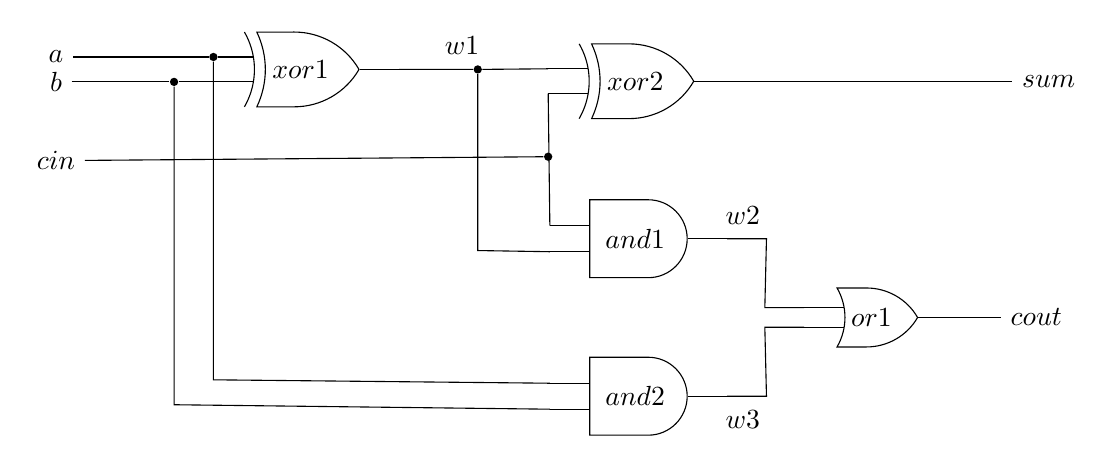
\begin{tikzpicture}[label distance=2mm]


        % XOR, WIRES AND CONNECTOR POINTS
        \node[my-xor-gate]     (XOR1)    at (0,0)                        {\normalsize $xor1$};
        \coordinate[my-branch] (XOR1IN1) at ($(XOR1.input 1) + (-.5, 0)$) {};
        \coordinate[]          (XOR1IN2) at ($(XOR1.input 2) + (-.5, 0)$) {};
        \coordinate[]          (XOR1OUT) at ($(XOR1.output)  + (.5, 0)$)  {};
        \draw (XOR1.input 1) -- (XOR1IN1);
        \draw (XOR1.input 2) -- (XOR1IN2);
        \draw (XOR1.output)  -- (XOR1OUT);

        % INPUTS
        \node[] (A)    at ($(XOR1IN1) + (-2, 0)$)  {\normalsize $a$};
        \node[] (B)    at ($(XOR1IN2) + (-2, 0)$)  {\normalsize $b$};
        \node[] (CIN)  at ($(XOR1IN2) + (-2, -1)$)  {\normalsize $cin$};

        % INTERNAL WIRE
        \node[my-branch] (W1)   at ($(XOR1OUT) + (1, 0)$)  {};
        
        % LABEL
        \node at ($(W1)   + (-.2, .3)$) {\normalsize $w1$};

        %B WIRE CONNECTOR POINTS
        \coordinate[my-branch]  (BCONNECT) at ($(XOR1IN2) + (-.5, 0)$) {};

        % INPUT CONNECTIONS
        \draw (A) -- (XOR1IN1);
        \draw (B) -- (BCONNECT);
        \draw (BCONNECT) -- (XOR1IN2);

        % XOR, WIRES AND CONNECTOR POINTS
        \node[my-xor-gate]     (XOR2)    at ($(XOR1OUT) + (3, -.15)$) {\normalsize $xor2$};
        \coordinate[]          (XOR2IN1) at ($(XOR2.input 1) + (-.5, 0)$) {};
        \coordinate[]          (XOR2IN2) at ($(XOR2.input 2) + (-.5, 0)$) {};
        \coordinate[]          (XOR2OUT) at ($(XOR2.output)  + (.5, 0)$)  {};
        \draw (XOR2.input 1) -- (XOR2IN1);
        \draw (XOR2.input 2) -- (XOR2IN2);
        \draw (XOR2.output)  -- (XOR2OUT);

        % CONNECTIONS
        \draw (XOR1OUT) -- (W1) -- (XOR2IN1);

        % AND, WIRES AND CONNECTOR POINTS
        \node[my-and-gate]     (AND1)    at ($(XOR2) + (0, -2)$) {\normalsize $and1$};
        \coordinate[]          (AND1IN1) at ($(AND1.input 1) + (-.5, 0)$) {};
        \coordinate[]          (AND1IN2) at ($(AND1.input 2) + (-.5, 0)$) {};
        \coordinate[]          (AND1OUT) at ($(AND1.output)  + (.5, 0)$)  {};
        \draw (AND1.input 1) -- (AND1IN1);
        \draw (AND1.input 2) -- (AND1IN2);
        \draw (AND1.output)  -- (AND1OUT);

        % AND, WIRES AND CONNECTOR POINTS
        \node[my-and-gate]     (AND2)    at ($(AND1) + (0, -2)$) {\normalsize $and2$};
        \coordinate[]          (AND2IN1) at ($(AND2.input 1) + (-.5, 0)$) {};
        \coordinate[]          (AND2IN2) at ($(AND2.input 2) + (-.5, 0)$) {};
        \coordinate[]          (AND2OUT) at ($(AND2.output)  + (.5, 0)$)  {};
        \draw (AND2.input 1) -- (AND2IN1);
        \draw (AND2.input 2) -- (AND2IN2);
        \draw (AND2.output)  -- (AND2OUT);

        % CONNECTIONS
        \node[my-branch] (CLKCONNECT) at ($(XOR2IN2) + (0, -.8)$)  {};

        % INTERNAL WIRES
        \draw (XOR1IN1) -- ($(XOR1IN1) + (0, -4.1)$) -- (AND2IN1);
        \draw (BCONNECT) -- ($(BCONNECT) + (0, -4.1)$) -- (AND2IN2);
        \draw (W1) -- ($(W1) + (0, -2.3)$) -- (AND1IN2);
        \draw (XOR2IN2) -- (AND1IN1);
        \draw (CIN) -- (CLKCONNECT);

        % OR, WIRES AND CONNECTOR POINTS
        \node[my-or-gate]      (OR1)    at ($(AND1) + (3, -1)$) {\normalsize $or1$};
        \coordinate[]          (OR1IN1) at ($(OR1.input 1) + (-.5, 0)$) {};
        \coordinate[]          (OR1IN2) at ($(OR1.input 2) + (-.5, 0)$) {};
        \coordinate[]          (OR1OUT) at ($(OR1.output)  + (.5, 0)$)  {};
        \draw (OR1.input 1) -- (OR1IN1);
        \draw (OR1.input 2) -- (OR1IN2);
        \draw (OR1.output)  -- (OR1OUT);

        % INTERNAL WIRES
        \draw (AND1OUT) -- ($(AND1OUT) + (.5, 0)$) -- ($(OR1IN1) + (-.5, 0)$) -- (OR1IN1);
        \draw (AND2OUT) -- ($(AND2OUT) + (.5, 0)$) -- ($(OR1IN2) + (-.5, 0)$) -- (OR1IN2);

        % LABEL
        \node at ($(AND1OUT)   + (.2, .3)$) {\normalsize $w2$};
        \node at ($(AND2OUT)   + (.2, -.3)$) {\normalsize $w3$};

        % OUTPUTS
        \node[] (SUM)    at ($(XOR2OUT) + (4, 0)$)  {\normalsize $sum$};
        \node[] (COUT)   at ($(OR1OUT) + (1, 0)$)  {\normalsize $cout$};

        % OUTPUT CONNECTIONS
        \draw (XOR2OUT) -- (SUM);
        \draw (OR1OUT) -- (COUT);

    \end{tikzpicture}
}

\end{document} 
